\begin{frame}
\begin{block}{\textbf{Question}}
How can we interpret these relationships geometrically?
\end{block}
\begin{block}{\textbf{Polytopes of probability distributions}}
Spaces of probability distributions and constraints placed upon them by linear transformations like G give rise to polytopes
\end{block}
\begin{block}{\textbf{Polytope}}
\begin{center}
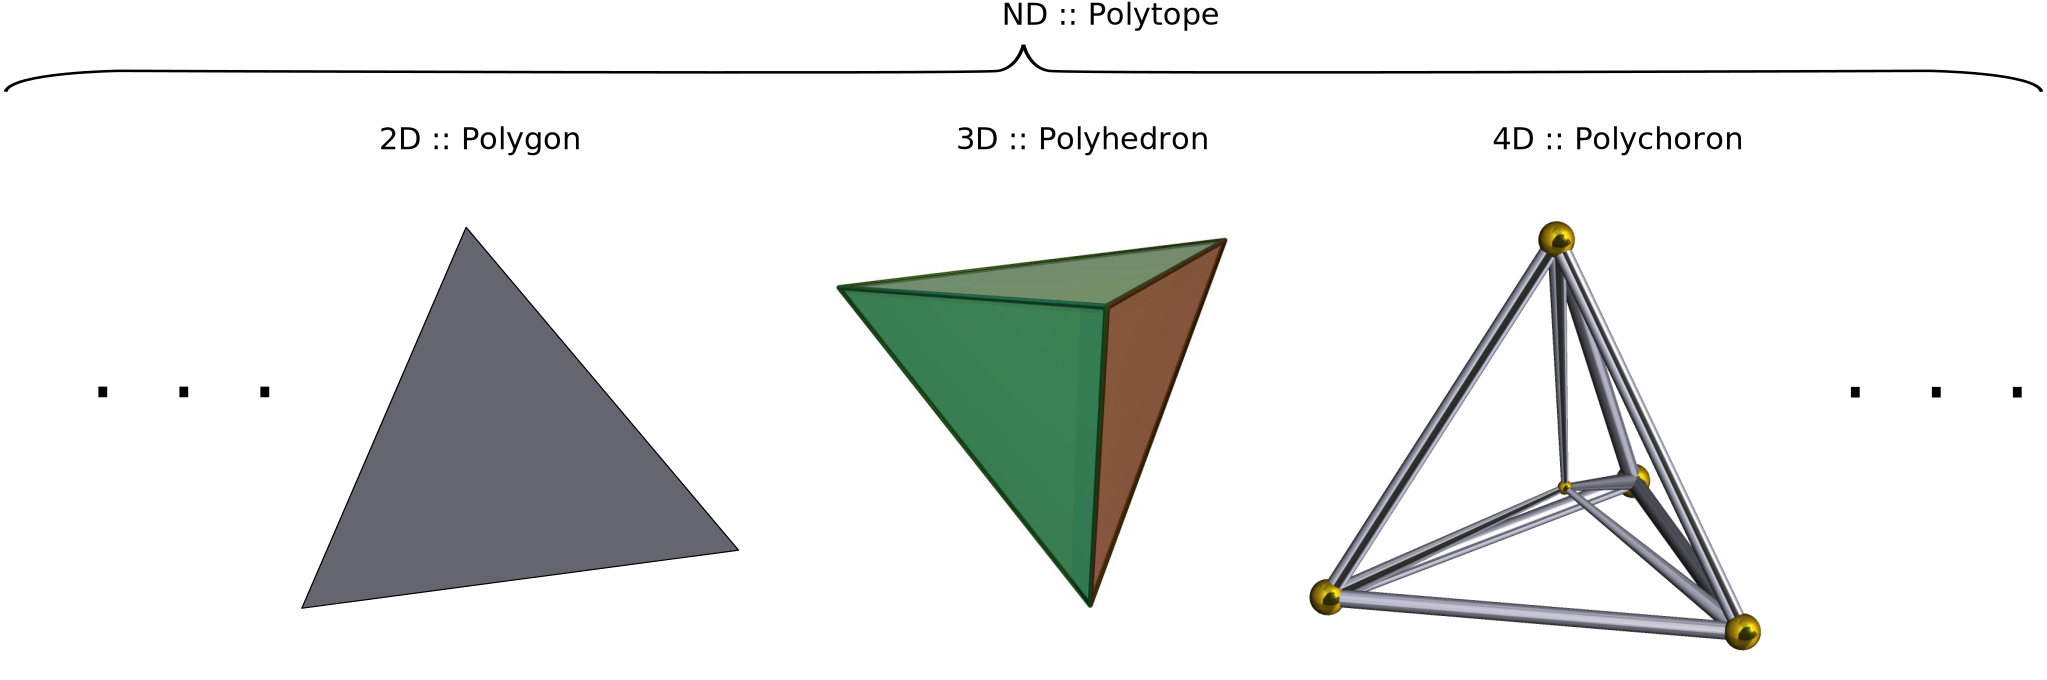
\includegraphics[width=0.9\textwidth]{fig/polytope.pdf}
\end{center}
\end{block}
\end{frame}

